\chapter{Introduction}
\label{introduction}
\section{Background and Motivation}
Board games are and have been a popular environment to test the capabilities of state-of-the-art artificial intelligence against human opponents. Many board games are widely known, making them a tangible measure of performance. The most prominent examples are the games of Chess and Go. For both, machines defeating the current best players has been representative of fundamental progress in computing.

IBM's "Deep Blue" defeated Gary Kasparov in 1996 \cite{higgins_brief_2017} by utilizing search to look ahead into the game tree and deliberate on the next move. This approach is a prime example for symbolic AI approaches, "good-old-fashioned-AI" ("GOFAI") \cite[p. 112f]{haugeland_artificial_1985}, which rely on logic and search on symbolic representations.

However, our limited ability to model the problem correctly and exhaustively severely constrains these knowledge-based approaches. For example, in the case of Deep Blue, it requires us to encode expert knowledge about chess in a heuristic function to evaluate the board. Only then we can search for actions that maximize this function. Problems with large complexity would require tremendous efforts, which just become infeasible at a certain point.

A different approach would be devising (general) methods to learn the necessary domain knowledge from scratch,  \emph{tabula rasa}. As Alan Turing put it:

\begin{quote}
    Instead of trying to produce a programme to simulate the adult mind, why not rather try to produce one which simulates the child's? If this were then subjected to an appropriate course of education one would obtain the adult brain. Presumably, the child-brain is something like a notebook as one buys it from the stationers. Rather little mechanism, and lots of blank sheets. [...] Our hope is that there is so little mechanism in the child-brain that something like it can be easily programmed.
    \cite{turing_icomputing_1950}
\end{quote}

The recent success of "AlphaGo" in 2016 against the long-time world champion Lee Sedol \cite{deepmind_match_nodate} in the game Go is a milestone that perfectly demonstrates this shift towards "bottom-up" or subsymbolic methods \cite{nilsson_artificial_1998}. The increasing availability of computational power (and data) has enabled two subsymbolic methods to find considerable success in unclaimed territory, such as computer vision or natural language processing. Namely, those are neural networks and (stochastic) gradient descent with backpropagation. Combined, they provide a general function approximator that can be trained in a process akin to the learning described by Turing.

In the case of Go, designing a powerful heuristic function was deemed impossible for humans. The team from DeepMind created AlphaGo using (deep) neural networks to learn an evaluation function based on an extensive database of expert moves. With the help of \textit{reinforcement learning} (RL), they improved this network even further by letting it play against itself. They used this trained function to then perform a look-ahead search on the game tree more effectively \cite{silver_mastering_2017}. Building on this success, DeepMind further improved the architecture. "AlphaGo Zero" and the generalization "AlphaZero" learn without the help of the database of expert moves. AlphaZero's learning process exclusively relies on deep reinforcement learning and \textit{self-play}.
Nevertheless, it surpassed the performance of AlphaGo significantly. Since then, the architecture has been applied to Chess, Shogi, and Atari games. "MuZero" went even further by removing the last piece of human knowledge in the system: the rules of the game \cite{schrittwieser_mastering_2020}.

\begin{figure}[H]
    \centering
    \subfloat[The original physical board of the game \cite{bradley_closed_2018}]{
        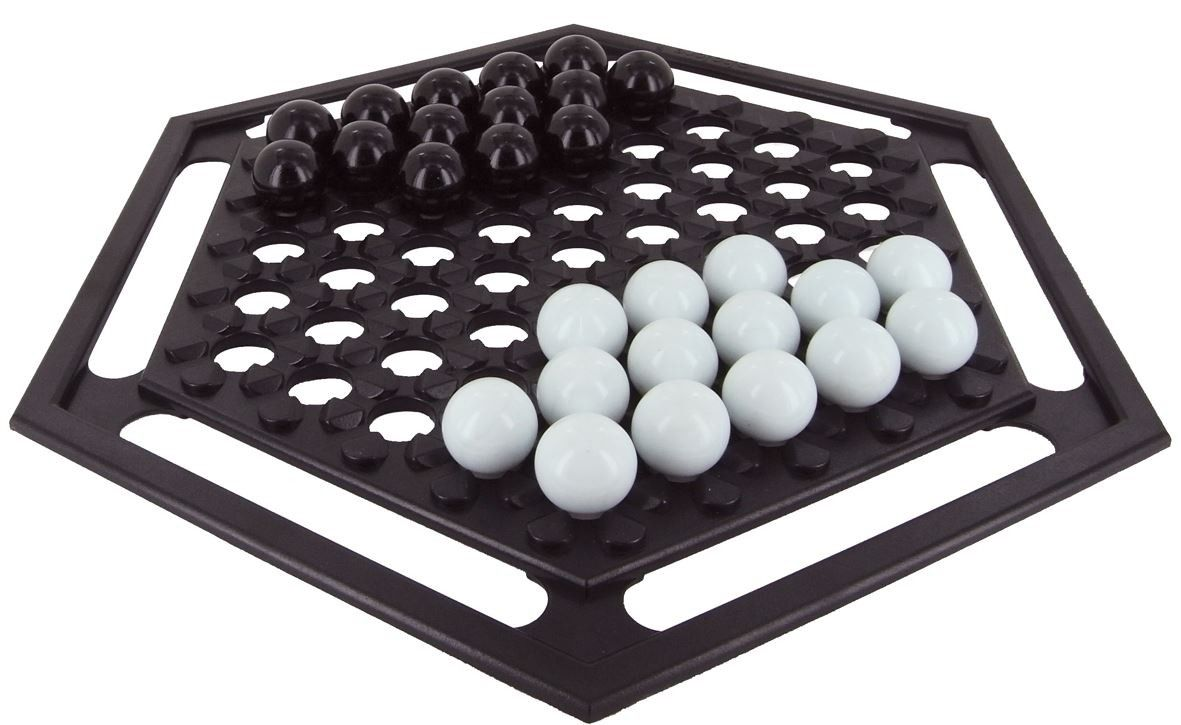
\includegraphics[height=4.5cm, keepaspectratio]{physical_abalone_board.jpg}
    }
    % \hfill
    \subfloat[Note the hexagonal shape of the board and the fields. A marble can be moved in upto six directions.]{
        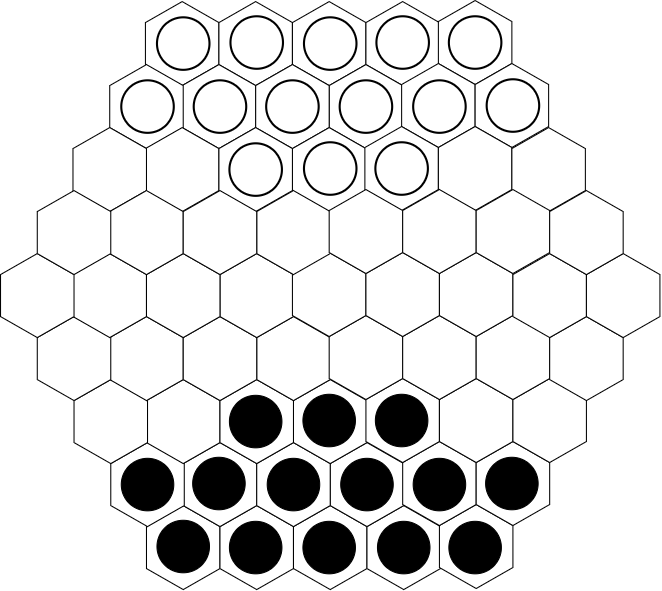
\includegraphics[height=4.5cm, keepaspectratio]{abalone_board_default.png}
    }
    \caption{The board of Abalone}
    \label{abalone_boards}
\end{figure}


At this point, our endeavor begins. The goal of this thesis is to apply the methods of AlphaZero to the game of Abalone. Abalone is a relatively young board game from 1987. The main variant is played by two players on a hexagonal board with 61 fields and 14 marbles for black and white, respectively. The game's goal is to push six of the opponent's marbles off the playing field.

Naturally, the question arises whether this goal is a worthwhile thing to do. Firstly, academic interest in Abalone has remained steady even though the game's popularity declined. However, the application of learning methods to Abalone is less explored, especially regarding the novel techniques introduced by AlphaZero.

Secondly, further investigating the applicability of RL is a relevant topic. Along with supervised and unsupervised learning, reinforcement learning is one of three basic machine learning paradigms \cite{noauthor_reinforcement_2022}. Aside from (super-) human performance in games \cite{mnih_human-level_2015, berner_dota_2019,vinyals_grandmaster_2019}, RL continues to find more industry application in areas like improving data center cooling at Google \cite{gamble_safety-first_2018} or content recommendation at Spotify \cite{jebara_for_2020} and Netflix \cite{siddiqi_ml_2019}. A very recent example is the floor planning for Google's latest TPU chip, which was aided by a deep RL algorithm \cite{mirhoseini_graph_2021}.

Additionally, RL finds application in robotic control. Through continuous trial and error learning robots learned to grasp \cite{pinto_supersizing_2016,zeng_learning_2018}, poke \cite{agrawal_learning_nodate} or to avoid obstacles \cite{kahn_uncertainty-aware_2017}. The learning was either performed in a simulated digital environment or through physical interaction.

\section{Research Goals}
First, let us establish the main research questions that will guide us throughout this thesis.

\paragraph{The first goal} is to apply the general framework of self-play learning outlined in "Mastering the game of Go without human knowledge" to the board game of Abalone. \cite{silver_mastering_2017} The original paper gives clear instructions on the theoretical groundwork for the system but omits clear instructions for the implementation. There is no open-source code provided.

\paragraph{The second goal} is to compare classical search-based methods to AlphaZero's deep reinforcement learning based on several criteria such as win/loss ratio and computational requirements.

\section{Structure}
% how are the goals achieved?
To provide the theoretical knowledge for understanding AlphaZero, the chapter \ref{background-theory} describes fundamentals in artificial intelligence, game-playing algorithms, (deep) reinforcement learning. The structure also mirrors the historical development of the methods.

The chapter \ref{abalone} uses some of the previously introduced knowledge to analyze Abalone and also provides insight into existing game-playing programs to gauge the state of the art.

The chapter \ref{system-architecture} is about the concrete implementation AlphaZero's methods for Abalone. It encompasses considerations about third-party software, Abalone specific adaptations, architecture, and algorithms.

Based on this software, chapter \ref{experiments-and-results} shows the experimental setup and the results for the implementation.

Lastly, in chapter \ref{conclusion} an evaluation of the results given and an outlook for the continuation of the work is given.
